 \سؤال{مشاهده‌ی فایل سیستم \lr{/proc}}
 
 \begin{enumerate}
 	\item با استفاده از دستور \lr{cd}  وارد شاخه‌ی \lr{/proc} می‌شویم.
 	
 	\begin{code}
 		> cd /proc
 	\end{code}
 
 	\item به کمک دستور \lr{ls} فایل‌های موجود در این شاخه را مشاهده می‌کنیم.
 	
 	\begin{code}
 		> ls
 	\end{code}
 	
 	\item فایل‌های موجود به همراه \lr{Process ID}ها
 	
 		\begin{figure}[!hbpt]
 			\centering
 			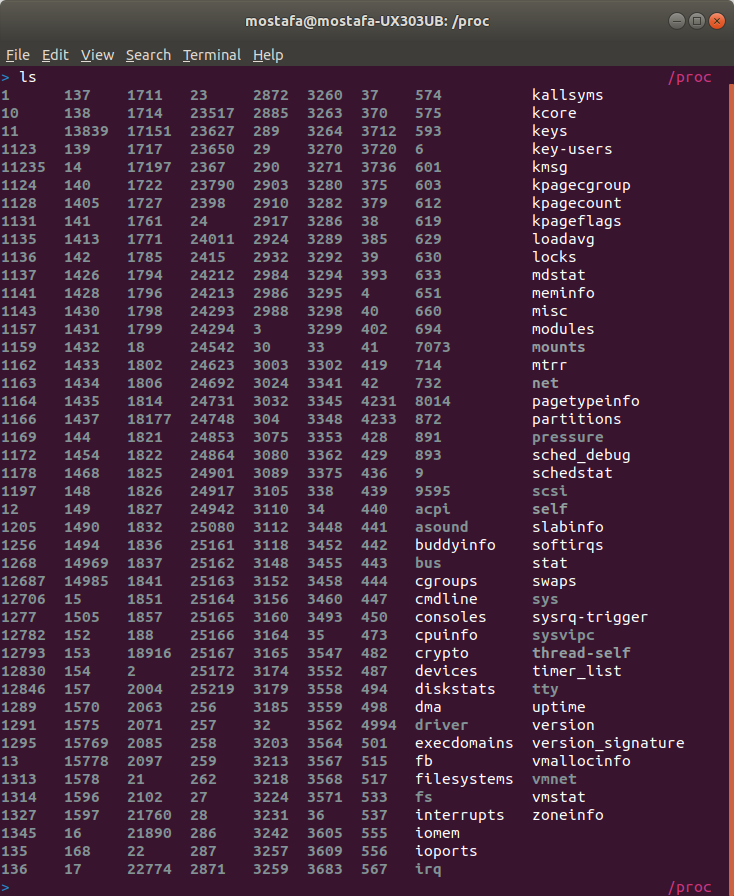
\includegraphics[scale=.35]{./img/1.png}
 			\caption{دستورهای سوال اول}
 		\end{figure}
\end{enumerate}

\newpage

\سؤال{مشاهده‌ی محتویات یک فایل در شاخه \lr{/proc}}

\begin{enumerate}
	\item محتوای فایل \lr{/proc/version}. 
	این فایل نام نسخه‌ی واقعی سیستم‌عامل را نشان نمی‌دهد، در عوض مشخصات مربوط به نسخه هسته‌ی لینوکس استفاده شده در توزیع و هم‌چنین نسخه‌ی کامپایلر \lr{GCC} که برای ساخت آن استفاده شده را نمایش می‌دهد.
	
	\begin{code}
		> cat version
		
		Linux version 5.4.0-42-generic (buildd@lgw01-amd64-023) (gcc version 7.5.0 		(Ubuntu
		
		 7.5.0-3ubuntu1~18.04)) \#46~18.04.1-Ubuntu SMP Fri Jul 10 07:21:24 UTC 2020
	\end{code}


	\item 
	
	
	\begin{itemize}
		\item \textbf{\lr{cmdline}}: در این فایل، پارامترهایی که سیستم هنگام \lr{boot} شدن از آن‌ها استفاده می‌کند را می‌توان بررسی کرد و هم‌چنین می‌توان دید که آیا شامل تغییرات است یا خیر.
		
		\item \textbf{cpuinfo}: نوع پردازنده و تعداد پردازنده‌های در حال اجرا را نمایش می‌دهد. 
		
		\item \textbf{diskstats}: آمارهای ورودی و خروجی مربوط به \lr{block devices} را نمایش می‌دهد.		
	\end{itemize}

	\item
	برنامه‌نویسی به زبان \lr{C++}
	
		\begin{Verbatim}[tabsize=4]
#include <iostream>
#include <fstream>
#include <string>
using namespace std;

int main() {
	string version;
	ifstream f;
	f.open("/proc/version", ios::in);
	getline(f, version);
	f.close();
	ofstream of;
	of.open("linux_version.txt", ios::out);
	of << version;
	of.close();
	return 0;
}

	\end{Verbatim}
	
	\item
	امکان نوشتن جمله‌ی دل‌خواه در آن وجود ندارد، زیرا این فایل از نوع \lr{read-only} است.
	
\end{enumerate}

\newpage
\سؤال{مشاهده‌ی وضعیت پردازه‌ها}

\begin{enumerate}
	\item 
	استفاده از دستور \lr{ls} در یکی از پردازه‌ها
	
	\begin{figure}[h!]
		\centering
		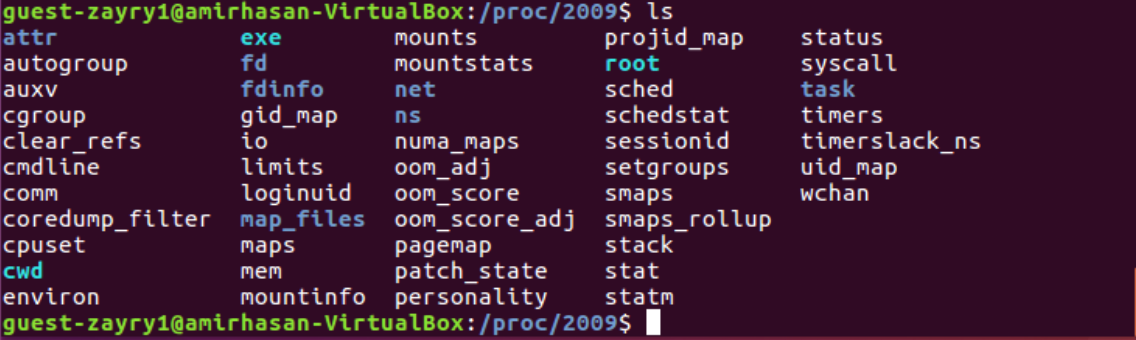
\includegraphics[scale=.4]{img/:proc:[pid].png}
	\end{figure}

	\item
توضیح	دستورها:
	\begin{itemize}
		\item \textbf{\lr{cmdline}}:
  این فایل تنها قابل خواندن بوده و در آن لیست آرگومان‌های داده شده به پردازه هنگام اجرای آن (\lr{argv}) قرار گرفته است که با $\textbackslash 0$ از هم جدا شده‌اند. برای پردازه‌های \lr{zombie} این فایل خالی است.
  
  \begin{figure}[h!]
  	\centering
  	
\includegraphics[scale=.4]{img/cmdline.png}
  \end{figure}
  
  		\item \textbf{\lr{environ}}:
  		 در این فایل لیست \lr{environment variable}هایی که در زمان اجرای پردازه وجود داشتند قرار دارد که با ($\textbackslash 0$) از هم جدا شده‌اند.
  		 \begin{figure}[h!]
  		 	\centering
  		 	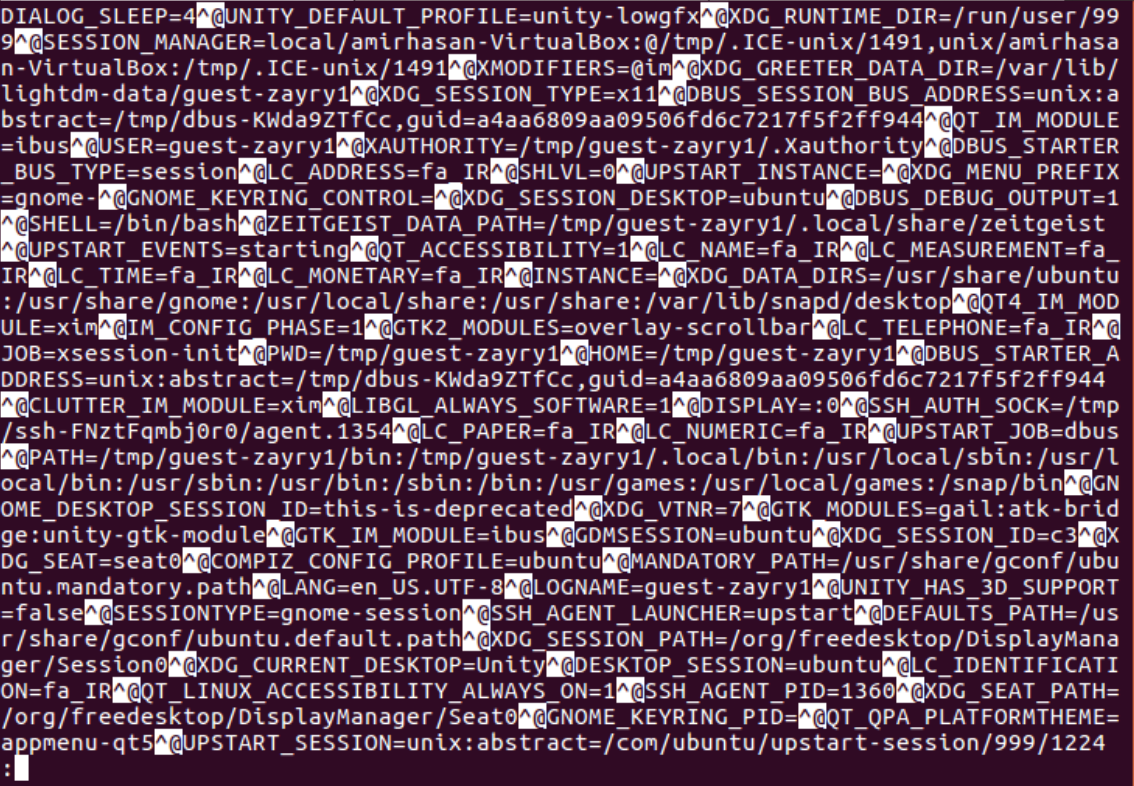
\includegraphics[scale=.4]{img/environ.png}
  		 \end{figure}
  	 
  		 \item \textbf{\lr{stat}}:
  		   اطلاعات مربوط به وضعیت پردازه شامل ۵۲ پارامتر از جمله شماره، نام، حالت (در حال اجرا، در صف انتظار،…)، شماره پردازه والد، اولویت، زمان شروع، حجم حافظه مجازی، و… که با \lr{space} جدا شده‌اند، در این فایل قرار دارد.
  		   
  		   \begin{figure}[h!]
  		   	\centering
  		   	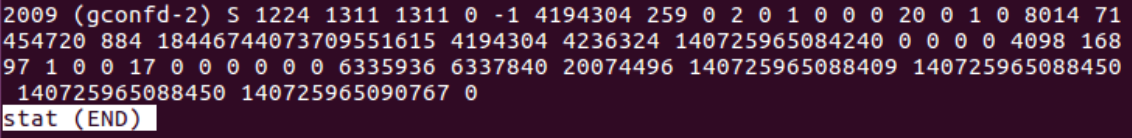
\includegraphics[scale=.4]{img/stat.png}
  		   \end{figure}
  		   
  		   \item \textbf{\lr{statm}}:
  		    اطلاعات مربوط به حافظه استفاده شده توسط پردازه بر حسب \lr{page} در این فایل قرار دارد.
  		      		   \begin{figure}[hbpt!]
  		    	\centering
  		    	
\includegraphics[scale=.4]{img/statm.png}
  		    \end{figure}
  		    \item \textbf{\lr{status}}:
  		     در این فایل اکثر اطلاعات موجود در \lr{stat} و \lr{statm} به صورت خواناتر برای انسان قرار دارد.
  		     
  		       		   \begin{figure}[h!]
  		     	\centering
  		     	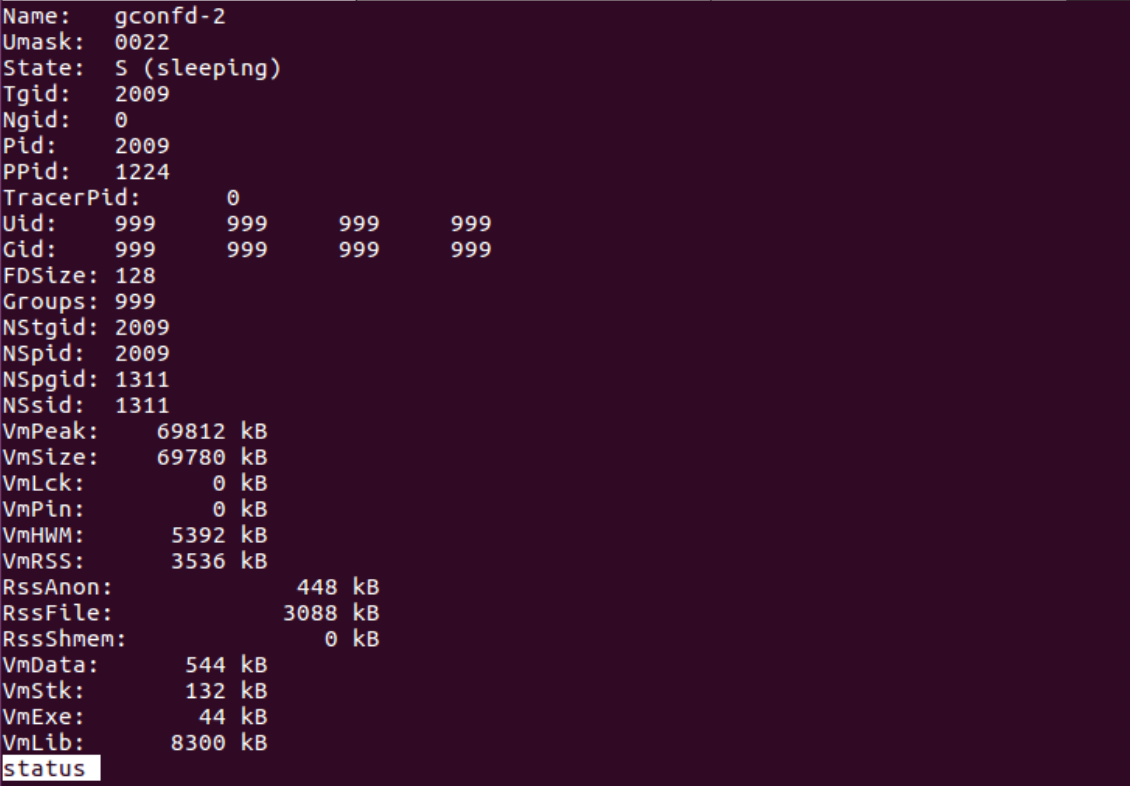
\includegraphics[scale=.4]{img/status.png}
  		     \end{figure}
  		     \item \textbf{\lr{cwd}}:
  		       این فایل یک \lr{symlink} است که به دایرکتوری کنونی پردازه اشاره می‌کند.
  		         		   \begin{figure}[hbpt!]
  		       	\centering
  		       	
\includegraphics[scale=.4]{img/cwd.png}
  		       \end{figure}
  		       \item \textbf{\lr{exe}}: 
  		       این فایل یک \lr{symlink} است که به فایل برنامه اجرا شده اشاره می‌کند.
  		         		   \begin{figure}[h!]
  		       	\centering
  		       	
\includegraphics[scale=.4]{img/exe.png}
  		       \end{figure}
  		      	\item \textbf{\lr{root}}: 
  		      	 این فایل یک \lr{symlink} است که به دایرکتوری \lr{root} مشخص شده برای پردازه اشاره می‌کند.
		   		   \begin{figure}[h!]
		 	\centering
		 	
\includegraphics[scale=.4]{img/root.png}
		 \end{figure}
	\end{itemize}
	\item اسکریپت برای دریافت لیست شماره‌ی پردازه‌های در حال اجرا
	
		\begin{Verbatim}[tabsize=4]
#!/bin/bash

cd /proc
re='^[0 - 9]+$'
for f in * ; do
	if [[ $f =~ $re ]] ; then
		read -r name < $f/status
		name=${name:5}
		echo "$f $name"
	fi
done
		\end{Verbatim}
	
	\item 
	برنامه‌ای که شماره‌ی یک پردازه را دریافت کند و اطلاعات آن را چاپ کد.
	
	\begin{Verbatim}[tabsize=4]
#!/bin/bash

pid=$1
re='^[0 - 9]+$'
if [[ $pid =~ $re ]] && [[ -d "/proc/$pid" ]] ; then
	read -r name < "/proc/$pid/status"
	name=${name:6}
	p=$(getconf PAGESIZE)
	s=$(cat "/proc/$pid/statm" | cut -d' ' -f 1)
	size=$(( $p * $s ))
	args=$(cat "/proc/$pid/cmdline" | cut -d $'\0' -f 2-)
	envvars=$(cat "/proc/$pid/environ")
	echo -e "Name: $name\nMemory: $size\nArgs: $args\nEnvironment Variables:\n$envvars"
else
	echo "There is no such process"
fi
	\end{Verbatim}
	
\end{enumerate}


